% Path diagram of the RI-CLPM (vignette ri-clpm).
\documentclass[tikz, border = 6pt]{standalone}
\usepackage{amsmath}
\usepackage{bm}
\usetikzlibrary{arrows.meta, positioning, calc}
\tikzset{
  lat/.style = {circle, draw, thick, minimum size = 12mm, inner sep = 0pt},
  obs/.style = {rectangle, draw, thick, minimum size = 10mm, inner sep = 1pt},
  noise/.style = {circle, draw, minimum size = 7mm, inner sep = 0pt},
  reg/.style = {-{Stealth[length = 2.5mm]}, thick},
  cov/.style = {{Stealth[length = 2mm]}-{Stealth[length = 2mm]}},
  var/.style = {cov, looseness = 5},
  lab/.style = {font = \footnotesize, fill = white, inner sep = 1pt},
  dots/.style = {font = \Large}
}
\begin{document}
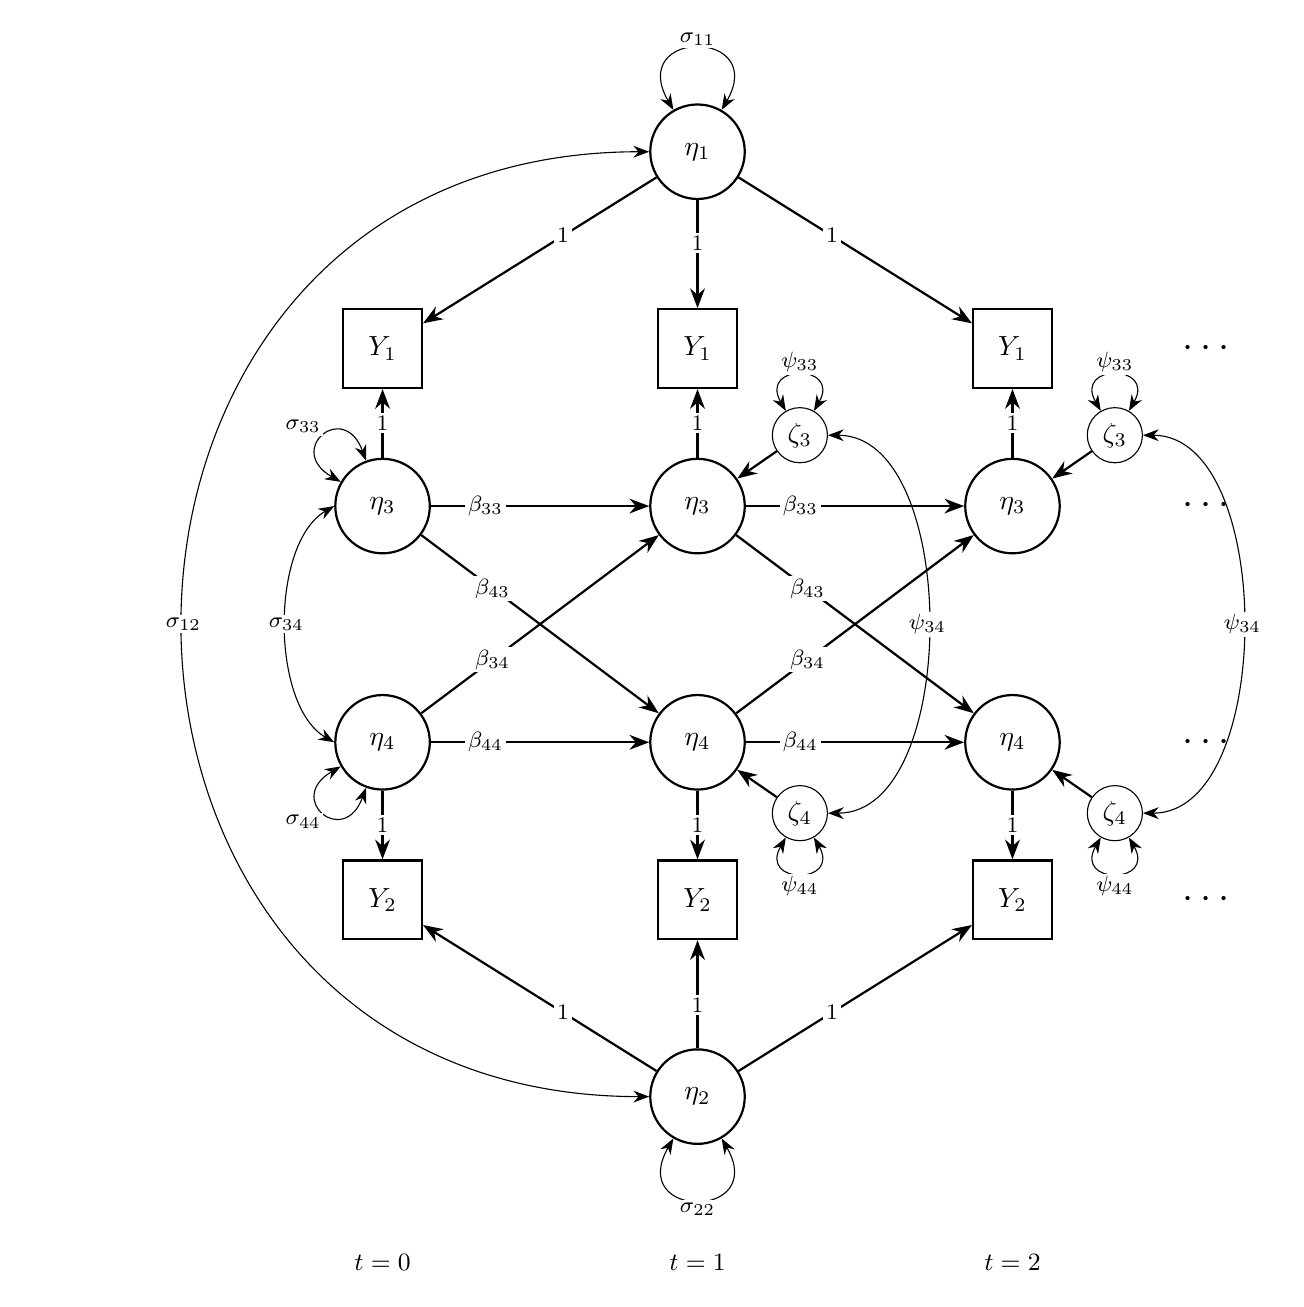
\begin{tikzpicture}
  % occasions
  \foreach \t/\x/\l in {1/0/0, 2/4/1, 3/8/2} {
    \node[obs] (y1\t) at (\x, 2) {$Y_{1}$};
    \node[lat] (w1\t) at (\x, 0) {$\eta_{3}$};
    \node[lat] (w2\t) at (\x, -3) {$\eta_{4}$};
    \node[obs] (y2\t) at (\x, -5) {$Y_{2}$};
    \draw[reg] (w1\t) -- node[lab] {1} (y1\t);
    \draw[reg] (w2\t) -- node[lab] {1} (y2\t);
    \node[font = \small] at (\x, -9.6) {$t = \l$};
  }
  % traits
  \node[lat] (t1) at (4, 4.5) {$\eta_{1}$};
  \node[lat] (t2) at (4, -7.5) {$\eta_{2}$};
  \foreach \t in {1, 2, 3} {
    \draw[reg] (t1) -- node[lab, pos = 0.4] {1} (y1\t);
    \draw[reg] (t2) -- node[lab, pos = 0.4] {1} (y2\t);
  }
  \draw[cov] (t1.west) .. controls (-4.5, 4.5) and (-4.5, -7.5) ..
    node[lab] {$\sigma_{12}$} (t2.west);
  % trait variances
  \draw[var] (t1.60) to[out = 60, in = 120]
    node[lab, above] {$\sigma_{11}$} (t1.120);
  \draw[var] (t2.240) to[out = 240, in = 300]
    node[lab, below] {$\sigma_{22}$} (t2.300);
  % within-person dynamics
  \foreach \s/\t in {1/2, 2/3} {
    \draw[reg] (w1\s) -- node[lab, pos = 0.25] {$\beta_{33}$} (w1\t);
    \draw[reg] (w2\s) -- node[lab, pos = 0.25] {$\beta_{44}$} (w2\t);
    \draw[reg] (w2\s) -- node[lab, pos = 0.3] {$\beta_{34}$} (w1\t);
    \draw[reg] (w1\s) -- node[lab, pos = 0.3] {$\beta_{43}$} (w2\t);
  }
  % process noise
  \foreach \t/\x in {2/4, 3/8} {
    \node[noise] (z1\t) at (\x + 1.3, 0.9) {$\zeta_{3}$};
    \node[noise] (z2\t) at (\x + 1.3, -3.9) {$\zeta_{4}$};
    \draw[reg] (z1\t) -- (w1\t);
    \draw[reg] (z2\t) -- (w2\t);
    \draw[cov] (z1\t.east) to[out = 0, in = 0, looseness = 0.9]
      node[lab] {$\psi_{34}$} (z2\t.east);
    \draw[var] (z1\t.60) to[out = 60, in = 120]
      node[lab, above] {$\psi_{33}$} (z1\t.120);
    \draw[var] (z2\t.240) to[out = 240, in = 300]
      node[lab, below] {$\psi_{44}$} (z2\t.300);
  }
  % initial within-person variances and covariance
  \draw[cov] (w11.west) to[out = 210, in = 150, looseness = 0.8]
    node[lab] {$\sigma_{34}$} (w21.west);
  \draw[var] (w11.110) to[out = 110, in = 150]
    node[lab, above left] {$\sigma_{33}$} (w11.150);
  \draw[var] (w21.210) to[out = 210, in = 250]
    node[lab, below left] {$\sigma_{44}$} (w21.250);
  % later occasions
  \foreach \r in {2, 0, -3, -5} {
    \node[dots] at (10.5, \r) {$\cdots$};
  }
\end{tikzpicture}
\end{document}